% !TeX document-id = {f19fb972-db1f-447e-9d78-531139c30778}
% !BIB program = biber

\documentclass[compress]{beamer}
%\documentclass[handout]{beamer}
\usepackage[T1]{fontenc}
\usetheme[block=fill,subsectionpage=progressbar,sectionpage=progressbar]{metropolis} 

\usepackage{wasysym}
\usepackage{etoolbox}
\usepackage[utf8]{inputenc}

\usepackage{threeparttable}
\usepackage{subcaption}

\usepackage{tikz-qtree}
\setbeamercovered{still covered={\opaqueness<1->{5}},again covered={\opaqueness<1->{100}}}


\usepackage{listings}

\lstset{
	basicstyle=\scriptsize\ttfamily,
	columns=flexible,
	breaklines=true,
	numbers=left,
	%stepsize=1,
	numberstyle=\tiny,
	backgroundcolor=\color[rgb]{0.85,0.90,1}
}



\lstnewenvironment{lstlistingoutput}{\lstset{basicstyle=\footnotesize\ttfamily,
		columns=flexible,
		breaklines=true,
		numbers=left,
		%stepsize=1,
		numberstyle=\tiny,
		backgroundcolor=\color[rgb]{.7,.7,.7}}}{}


\lstnewenvironment{lstlistingoutputtiny}{\lstset{basicstyle=\tiny\ttfamily,
		columns=flexible,
		breaklines=true,
		numbers=left,
		%stepsize=1,
		numberstyle=\tiny,
		backgroundcolor=\color[rgb]{.7,.7,.7}}}{}



\usepackage[american]{babel}
\usepackage{csquotes}
\usepackage[style=apa, backend = biber]{biblatex}
\DeclareLanguageMapping{american}{american-UoN}
\addbibresource{../../bdaca.bib}
\renewcommand*{\bibfont}{\tiny}

\usepackage{tikz}
\usetikzlibrary{shapes,arrows,matrix}
\usepackage{multicol}

\usepackage{subcaption}

\usepackage{booktabs}
\usepackage{graphicx}



\makeatletter
\setbeamertemplate{headline}{%
	\begin{beamercolorbox}[colsep=1.5pt]{upper separation line head}
	\end{beamercolorbox}
	\begin{beamercolorbox}{section in head/foot}
		\vskip2pt\insertnavigation{\paperwidth}\vskip2pt
	\end{beamercolorbox}%
	\begin{beamercolorbox}[colsep=1.5pt]{lower separation line head}
	\end{beamercolorbox}
}
\makeatother



\setbeamercolor{section in head/foot}{fg=normal text.bg, bg=structure.fg}



\newcommand{\question}[1]{
	\begin{frame}[plain]
		\begin{columns}
			\column{.3\textwidth}
			\makebox[\columnwidth]{
				
\includegraphics[width=\columnwidth,height=\paperheight,keepaspectratio]{../../pictures/mannetje.png}}
			\column{.7\textwidth}
			\large
			\textcolor{orange}{\textbf{\emph{#1}}}
		\end{columns}
\end{frame}}



\title[Big Data and Automated Content Analysis]{\textbf{Big Data \& Automated Content Analysis} \\ Week 4 -- Wednesday: »Data Wrangling«}
\author[Anne Kroon]{Anne Kroon \\ ~ \\ \footnotesize{a.c.kroon@uva.nl \\@annekroon}}
\date{19 April 2021}
\institute[UvA]{Afdeling Communicatiewetenschap \\Universiteit van Amsterdam}

\begin{document}

\begin{frame}{}
	\titlepage
\end{frame}

\begin{frame}{Today}
	\tableofcontents
\end{frame}


\begin{frame}[standout]
	Everything clear from last week?
\end{frame}




\section{Statistics in Python}
\subsection{General considerations}


\begin{frame}{General considerations}
So you retrieved some cool data from a JSON API, selected some interesting key-value pairs, and maybe also created a rectangular dataframe.

Of course, you can always export to .csv and use R or Stata or SPSS or whatever\ldots

\vspace{1cm}
\pause

~~~~~~~~~~~~~~~~ \Huge{BUT:}
\end{frame}


\begin{frame}{Reasons for not exporting and analyzing somewhere else}
\begin{itemize}
	\item the dataset might be too big
	\item it's cumbersome and wastes your time
	\item it may introduce errors and makes it harder to reproduce
	\item you want to learn Python ;-)
\end{itemize}
\end{frame}


\begin{frame}{What statistics capabilities does Python have?}
	
\begin{itemize}
	\item Basically all standard stuff (bivariate and multivariate statistics) you know from SPSS
	\item Nowadays: also  really advanced stuff (e.g., time series analysis via \texttt{statsmodels}; structural equation modelling via \texttt{semopy}; \ldots)
	\item Yet, for some really specific advanced statistical models, you may want to look somewhere else (else==R)
	
\end{itemize}
\end{frame}





\subsection{Useful packages}


\begin{frame}{Useful packages}
	\begin{description}
		\item[numpy] (numerical python) Provides a lot of frequently used functions, like mean, standard deviation, correlation, \ldots
		\item[scipy] (scientic python) More of that ;-)
		\item[statsmodels] Statistical models (e.g., regression or time series)
		\item[matplotlib] Plotting
		\item[seaborn] Even nicer plotting
		\item[plot.ly] Also nicer plotting (+ interactive)
	\end{description}
\end{frame}


\begin{frame}[fragile]{Example 1: basic numpy}
\begin{lstlisting}
import numpy as np
x = [1,2,3,4,3,2]
y = [2,2,4,3,4,2]
z = [9.7, 10.2, 1.2, 3.3, 2.2, 55.6]
np.mean(x)
\end{lstlisting}
\begin{lstlistingoutput}
2.5
\end{lstlistingoutput}
\begin{lstlisting}
np.std(x)
\end{lstlisting}
\begin{lstlistingoutput}
0.9574271077563381
\end{lstlistingoutput}

\begin{lstlisting}
np.corrcoef([x,y,z])
\end{lstlisting}

\begin{lstlistingoutput}
array([[ 1.        ,  0.67883359, -0.37256219],
       [ 0.67883359,  1.        , -0.56886529],
       [-0.37256219, -0.56886529,  1.        ]])
\end{lstlistingoutput}

\end{frame}




\begin{frame}[fragile]{Example 1: basic numpy}
\begin{lstlisting}
from scipy.stats import skew, kurtosis
for li in (x,y):
    print(f"Skewness of {li}: {skew(li)}. Kurtosis: {kurtosis(li)}")
\end{lstlisting}
\begin{lstlistingoutput}
Skewness of [1, 2, 3, 4, 3, 2]: 0.0. Kurtosis: -0.942148760330578
Skewness of [2, 2, 4, 3, 4, 2]: 0.3329709512140237. Kurtosis: -1.6765755053507732
\end{lstlistingoutput}

\begin{lstlisting}
from scipy.stats import kendalltau, spearmanr, pearsonr
print(kendalltau(x,y), spearmanr(x,y), pearsonr(x,y))
\end{lstlisting}
\begin{lstlistingoutput}
KendalltauResult(correlation=0.5853694070049636, pvalue=0.1373671546813069) SpearmanrResult(correlation=0.7627700713964739, pvalue=0.0777416409478997) (0.6788335930269976, 0.13815797750490888)
\end{lstlistingoutput}

\end{frame}



\begin{frame}{Characteristics}
\begin{itemize}
	\item Operates (also) on simple lists
	\item Returns output in standard datatypes (you can print it, store it, calculate with it, \ldots)
	\item it's fast! \texttt{np.mean(x)} is faster than \texttt{sum(x)/len(x)}
	\item it is more accurate (less rounding errors) 
\end{itemize}
\end{frame}





\begin{frame}[fragile]{Example 2: basic plotting}
\begin{lstlisting}
import matplotlib.pyplot as plt
x = [1,2,3,4,3,2]
y = [2,2,4,3,4,2]
plt.hist(x)
plt.plot(x,y)
plt.scatter(x,y)
\end{lstlisting}


\begin{figure}[h]
	\centering
	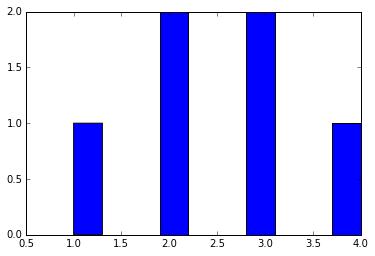
\includegraphics[width=.3\linewidth]{../../pictures/plthist}\hfill
	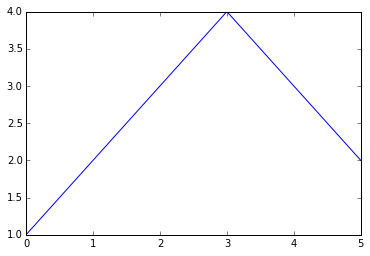
\includegraphics[width=.3\linewidth]{../../pictures/pltplot}\hfill
	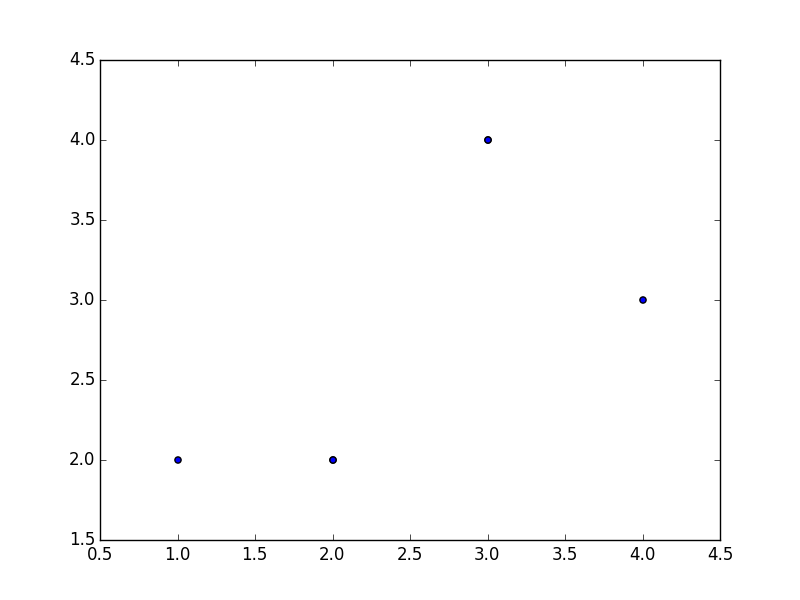
\includegraphics[width=.3\linewidth]{../../pictures/pltscatter}
	\caption{\label{fig:matplotlib}Examples of plots generated with \texttt{matplotlib}}
\end{figure}

\end{frame}





\section{Pandas basics}
\subsection{Working with dataframes}





\begin{frame}{When to use dataframes}
	\footnotesize
	\begin{columns}[t]
		\column{.5\textwidth}
		
		\begin{block}<1->{Lists, dicts, generators}
		pro:
		\begin{itemize}
			\item flexible (especially dicts!)
			\item fast
			\item straightforward and easy to understand
		\end{itemize}
		con:
		\begin{itemize}
			\item if your data is a table, modeling this as, e.g., lists of lists feels unintuitive
			\item very low-level: you need to do much stuff `by hand'
		\end{itemize}
		
		\end{block}
		
		\column{.5\textwidth}
		
		\begin{block}<2->{Pandas dataframes}
			pro:
			\begin{itemize}
				\item like an R dataframe or a STATA or SPSS dataset
				\item many built-in methods for statistics, plotting, grouping, subsetting, \ldots)
			\end{itemize}
			con:
			\begin{itemize}
				\item `overkill' if you just want correlate two lists or so
				\item unsuitable for REALLY large datasets
			\end{itemize}
			
		\end{block}
		
	\end{columns}
	
\end{frame}







\subsection{Plotting and calculating with Pandas}


\begin{frame}{}

More examples here: \url{https://github.com/annekroon/bdaca-6ec/tree/master/6ec/week04/examples/basic_statistics.ipynb}


\end{frame}


\begin{frame}[fragile]{OLS regression in pandas}
\begin{lstlisting}
import pandas as pd
import statsmodels.formula.api as smf 

df = pd.DataFrame({'income': [10,20,30,40,50], 'age': [20, 30, 10, 40, 50], 'facebooklikes': [32, 234, 23, 23, 42523]})

myfittedregression = smf.ols(formula='income ~ age + facebooklikes', data=df).fit()
print(myfittedregression.summary())
\end{lstlisting}
	
\end{frame}


\begin{frame}[plain,fragile]{}

\begin{lstlistingoutputtiny}
OLS Regression Results                            
==============================================================================
Dep. Variable:                 income   R-squared:                       0.579
Model:                            OLS   Adj. R-squared:                  0.158
Method:                 Least Squares   F-statistic:                     1.375
Date:                Mon, 05 Mar 2018   Prob (F-statistic):              0.421
Time:                        18:07:29   Log-Likelihood:                -18.178
No. Observations:                   5   AIC:                             42.36
Df Residuals:                       2   BIC:                             41.19
Df Model:                           2                                         
Covariance Type:            nonrobust                                         
=================================================================================
coef    std err          t      P>|t|      [95.0% Conf. Int.]
---------------------------------------------------------------------------------
Intercept        14.9525     17.764      0.842      0.489       -61.481    91.386
age               0.4012      0.650      0.617      0.600        -2.394     3.197
facebooklikes     0.0004      0.001      0.650      0.583        -0.002     0.003
==============================================================================
Omnibus:                          nan   Durbin-Watson:                   1.061
Prob(Omnibus):                    nan   Jarque-Bera (JB):                0.498
Skew:                          -0.123   Prob(JB):                        0.780
Kurtosis:                       1.474   Cond. No.                     5.21e+04
==============================================================================

\end{lstlistingoutputtiny}
	
\end{frame}




\begin{frame}[fragile]{Other cool df operations}
\begin{description}
	\item[df{['age']}.plot()] to plot a column
	\item[df{['age']}.describe()] to get descriptive statistics 
	\item[df{['age']}.value\_counts()] to get a frequency table
\end{description}
and MANY more\ldots
	
\end{frame}




\begin{frame}[fragile]{Recoding and transforming}
	\small
To transform your data, you can use (amongst others) \texttt{.apply()}, \texttt{.applymap()}, and \texttt{.map()} or the .str.XXX() methods:

\begin{lstlisting}
df['is_center'] = df['hood'].str.contains('[cC]enter')
\end{lstlisting}
or define your own function:
\begin{lstlisting}
def is_center(x):
    return int(x.lower().find('center') > -1)
    
df['is_center'] = df['hood'].map(is_center)
\end{lstlisting}
or use a throwaway-function:
\begin{lstlisting}
df['is_center'] = df['hood'].map(lambda x: int(x.lower().find('center') > -1))
\end{lstlisting}

or use \texttt{.replace()} for simple recoding based on lists or a dict (not shown, see \url{https://pandas.pydata.org/pandas-docs/stable/reference/api/pandas.DataFrame.replace.html})



\end{frame}



\section{Pandas II: Data wrangling}
\subsection{Subsetting and slicing}

\begin{frame}[plain]
Subsetting and slicing
\end{frame}

\begin{frame}{Subsetting and slicing}
Recap:
\begin{itemize}[<+->]
	\item \texttt{[0:5]} to get elements 0, 1, 2, 3, 4 (works with lists, dataframes \ldots)
	\item \texttt{mydict['keyicareabout']} to get value (content) associated with the key
\end{itemize}

\pause

And therefore, also:

\begin{itemize}[<+->]
	\item \texttt{df[['col1', 'col2']]} to get only these two columns of a dataset
	\item \texttt{df[df['col1']=='whatever']} to get only the rows in which col1 is identical to the string 'whatever'
	\item \texttt{df[df['col2']>0]} to get only the rows in which col2 is a number bigger than 0
\end{itemize}


\end{frame}



\begin{frame}{More subsetting}
	To get a apecific row and/or column, you can use \texttt{.iloc[]} and \texttt{.loc[]}
\begin{itemize}[<+->]
	\item \texttt{.iloc[]} takes an int (the row/column numbers, \texttt{.loc[]} the names)
	\item \texttt{df.iloc[0,5]} to get row 0, column 5
	\item \texttt{df.loc[0,'what']} to get row 0, column 'what'
\end{itemize}

\end{frame}


{\setbeamercolor{background canvas}{bg=black}
\begin{frame}[plain]
\makebox[\linewidth]{
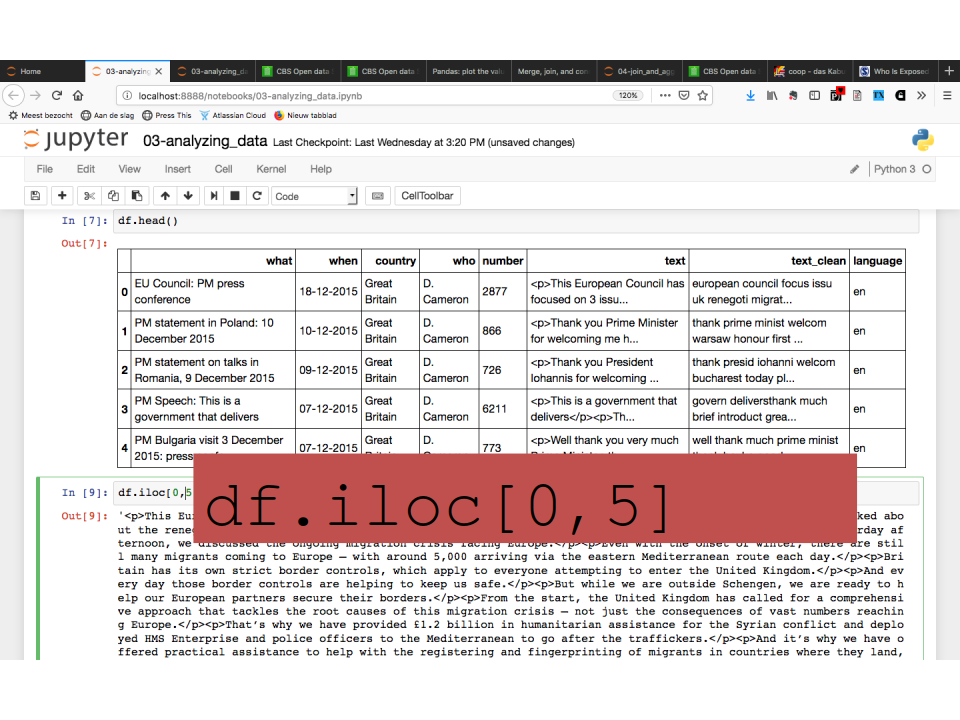
\includegraphics[width=\paperwidth,height=\paperheight,keepaspectratio]{../../pictures/pandas-iloc.png}}
\end{frame}

\begin{frame}[plain]
\makebox[\linewidth]{
	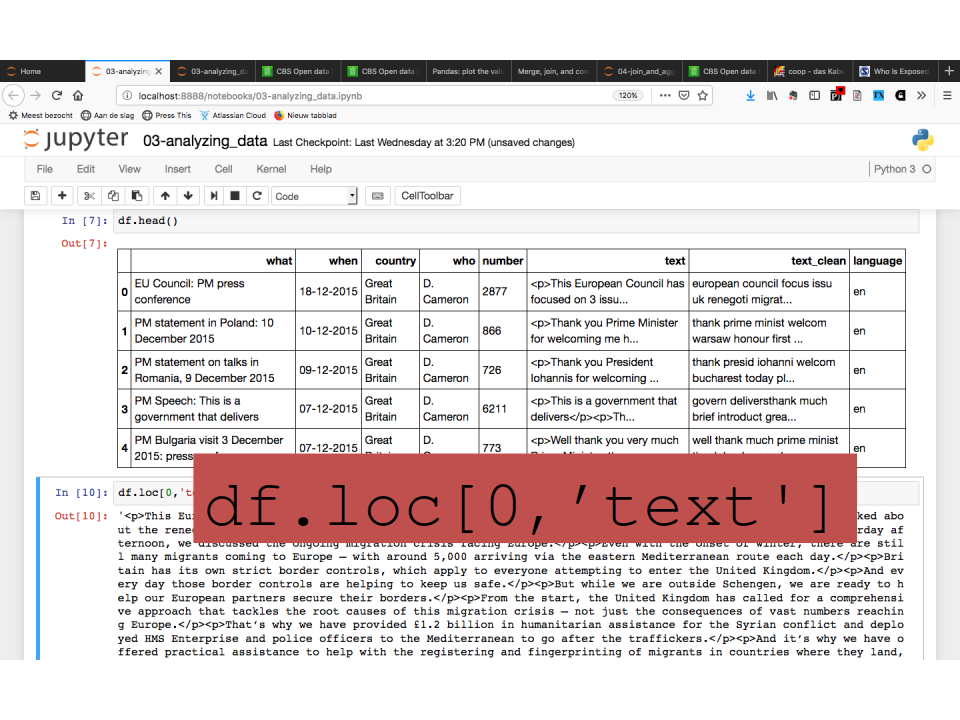
\includegraphics[width=\paperwidth,height=\paperheight,keepaspectratio]{../../pictures/pandas-loc.png}}
\end{frame}
}


\begin{frame}{Advanced Example}
Out of a dataset with $1,000$ speeches, get the one that talks most about [Tt]error
\begin{enumerate}[<+->]
	\item We create a new column to count how many a word is mentioned: \\ 
	\texttt{df['terror'] = df['speech'].str.count('[Tt]error')}
	\item We do \\ \texttt{df.iloc[\textcolor{red}{df['terror'].idxmax()}]}
	\item That works because df.iloc[] expects an integer to identify the row number, and \texttt{\textcolor{red}{df['terror'].idxmax()}} returns an integer (687 in our case)
\end{enumerate}

\end{frame}

{\setbeamercolor{background canvas}{bg=black}
	\begin{frame}[plain]
	\makebox[\linewidth]{
		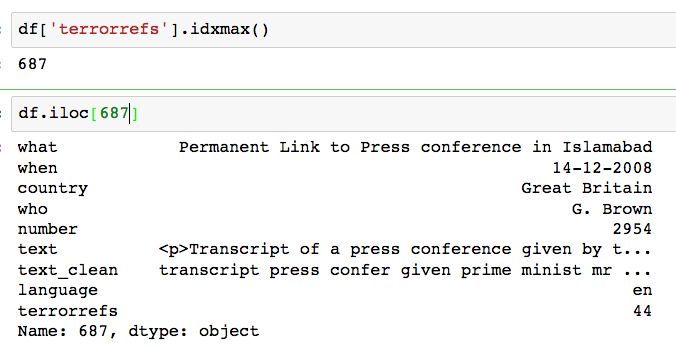
\includegraphics[width=\paperwidth,height=\paperheight,keepaspectratio]{../../pictures/pandas-idxmax.png}}
\end{frame}
}




\begin{frame}{A note on hard-coded ``magic numbers'' }
	Hard-coding ``magic numbers'' like \texttt{687} or \texttt{(0, 5)} in the examples above is really bad style and should be avoided. Always \emph{calculate} them from your data.
	
	If you \emph{really} cannot do this, define them as a constant at the beginning of your script: \texttt{ROW\_WITH\_CORRUPT\_DATA=438}.)
\end{frame}



\subsection{Joining and Merging}

\begin{frame}{Joining and Merging}
\begin{block}{Typical scenario}
	\begin{itemize}
		\item You have two datasets that share one column
		\item For instance, data from \url{www.cbs.nl}: one with economic indicators, one with social indicators
		\item You want to make one dataframe
	\end{itemize}
\end{block}
\end{frame}




{\setbeamercolor{background canvas}{bg=black}
	\begin{frame}[plain]
	\makebox[\linewidth]{
		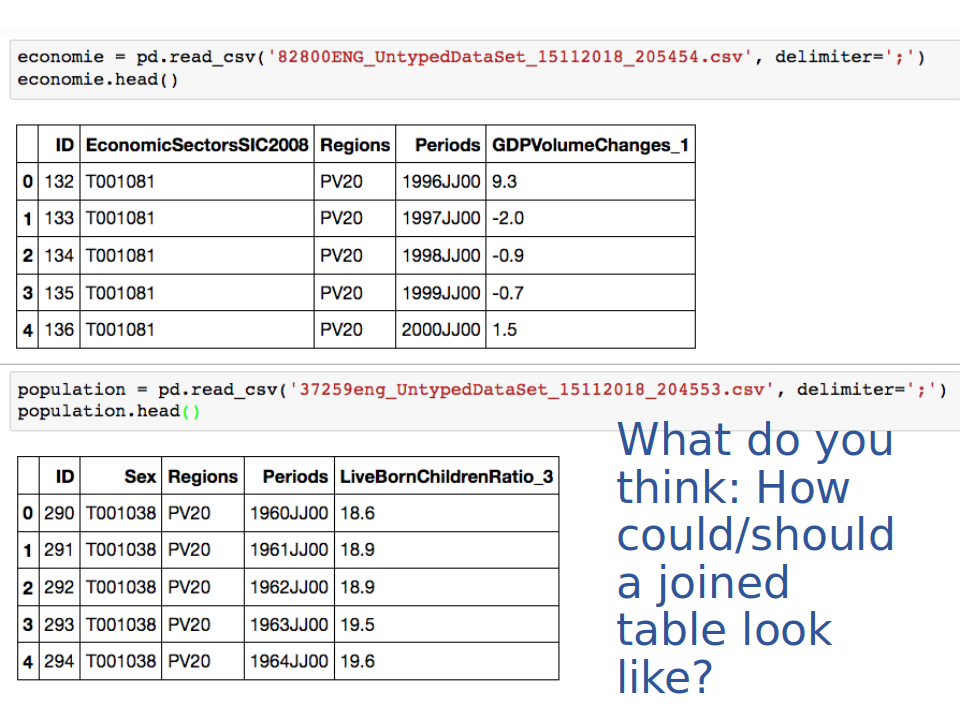
\includegraphics[width=\paperwidth,height=\paperheight,keepaspectratio]{../../pictures/pandas-join1.png}}
\end{frame}
	\begin{frame}[plain]
\makebox[\linewidth]{
	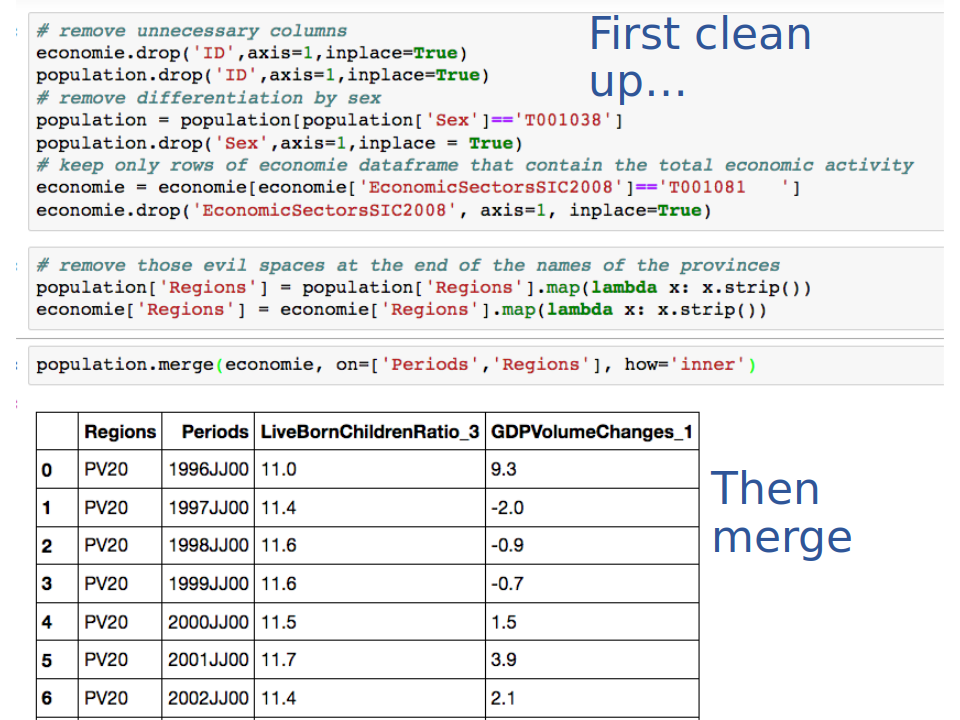
\includegraphics[width=\paperwidth,height=\paperheight,keepaspectratio]{../../pictures/pandas-join2.png}}
\end{frame}
}

\begin{frame}[fragile]{On what do you want to merge/join?}
Standard behavior of.join(): on the row index  (i.e., the row number, unless
you changed it to sth else like a date)
\begin{lstlisting}
df3 = df1.join(df2)
\end{lstlisting}
\pause
But that’s only meaningful if the indices of df1 and df2 mean the same. Therefore you can also join on a column if both dfs have it:
\begin{lstlisting}
df3 = df1.merge(df2, on='Regions')
\end{lstlisting}
\pause
\texttt{.merge()} is the more powerful tool, \texttt{.join()} is a bit easier when joining ion indices.
\end{frame}

\begin{frame}[fragile]{Inner, Outer, Left, and Right}
Main question: What do you want to do with keys that exist only in one of the  dataframes? \\
\pause
\vfill
\texttt{df3 = df1.join(df2, how='xxx')}\\
\vfill

\makebox[\linewidth]{
	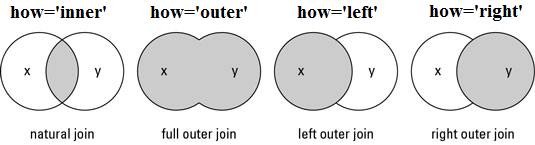
\includegraphics[width=\paperwidth,height=\paperheight,keepaspectratio]{../../pictures/join.png}}
\end{frame}


\subsection{Aggregation}
\begin{frame}[plain]
Aggregation
\end{frame}

\begin{frame}{An example}
\begin{itemize}
\item Suppose you have two dataframes, both containing information on something  per region per year.
\item 	You want to merge (join) the two, however, in one of them, the information is also split up by age groups. You don’t want that.
\item 	How do you bring these rows back to one row? With \texttt{.agg()}!
\end{itemize}

\end{frame}


\begin{frame}{.agg()}
\begin{itemize}[<+->]
\item Very useful after a \texttt{.groupby()}
\item Takes a function as argument: \\	\texttt{df2 = df.groupby('region').agg(sum)}
\item Or multiple functions: \\ \texttt{df2 = df.groupby('region').agg([sum, np.mean])}
\item $\rightarrow$ yes, you could do \texttt{.describe()}, but \texttt{.agg()} is more flexible	
\end{itemize}
\end{frame}


\begin{frame}[standout]
Exercise\\
Can you understand the code (join\_and\_aggregate.ipynb) and explain to a classmate?

\url{https://github.com/annekroon/bdaca-6ec/tree/master/6ec/week04/exercises}


\end{frame}


\section{Next steps}
\begin{frame}{}
\begin{block}{Friday: Visualization in Python}
	\begin{itemize}
	\item First part: I'll walk you through different libraries
	\item Second part: Take a dataset of your choice and try to apply the techniques discussed.
	\end{itemize}
\end{block}

\begin{block}{Take home exam: Thursday 29 April to Monday evening 3 May}
Three parts: 
\begin{enumerate}
	\item Essay-like literature question
	\item Programming task (``analyze this dataset'', ``write a program that does X'')
	\item Methods question (``You do not have to implement this right now, but how would you\ldots'')
\end{enumerate}
\end{block}
\end{frame}



\end{document}


